\section{Optimum Filters}
An optimum filter minimizes the mean-square error $\xi = E\left(|e(n)|^2\right) \quad x(n)=d(n)+v(n) \quad e(n) = d(n) - \tilde{d}(n)$\\
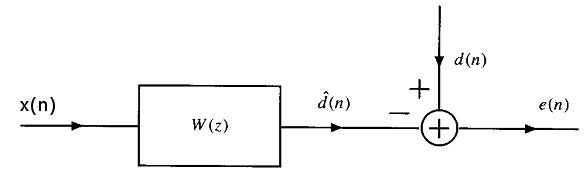
\includegraphics[width=9cm]{../TSM_StatDig/bilder/optimumFilter.jpg}\\
The minimal error is \textbf{always orthogonal} to the data: $E\{e(n)x^*(n-k)\}=0$ $\forall$ $k\in[0,p-1]$

\subsection{Wiener FIR Filter \hayes{337}}
\begin{minipage}{10cm}
\begin{tabbing}

Wiener-Hopf equations: \= $\sum \limits_{l=0}^{p-1} w(l)r_x(k-l)=r_{dx}(k)$; $\forall$ $k\in[0,p-1]$ \\
Correlations:  \>
						$r_x(k)=E \{ x(n)x^{*}(n-k) \}$ \\
\>						$r_{dx}(k)=E\{d(n)x^{*}(n-k)\}$ \\
Minimum Error: \>		$\xi_{min}=r_d(0)-\sum \limits_{l=0}^l w(l)r_{dx}^{*}(l)$
\end{tabbing}
\end{minipage}
\begin{minipage}{10cm}
$\small
\underbrace{\begin{bmatrix}
    		r_x[0] & r_x^*[1] & \hdots & r_x^*[p-1] \\
    		r_x[1] & r_x[0] & \hdots & r_x^*[p-2] \\
    		\vdots & \vdots & \ddots & \vdots \\
    		r_x[p-1] & r_x[p-2] & \hdots & r_x[0] \\
		\end{bmatrix}  }_{R_x} \cdot \underbrace{\begin{bmatrix}
    		w(0) \\
    		w(1) \\
    		\vdots \\
    		w(p-1)
		\end{bmatrix}  }_{w}= \underbrace{\begin{bmatrix}
    		 r_{dx}[0]\\
    		 r_{dx}[1]\\
    		\vdots \\
    		 r_{dx}[p-1]\\
		\end{bmatrix}}_{r_{dx}}
		 $$ \normalsize	 $\\
$$R_x \cdot w =r_{dx}$$
\end{minipage}
\begin{minipage}{7.5cm}
\subsubsection{Filtering \hayes{339}}
The input signal is $x(n)=d(n)+v(n)$. Because the noise and data signals are uncorrollated and the noise has zero mean, the Wiener-Hopf equation simplifies as follows:\\
$r_x(k)=r_d(k)+r_v(k)$\\
$r_{dx}(k)=r_d(k) \hspace{1.5cm} \rightarrow [R_d + R_v]\cdot w = r_d$\\
 with $R_v=\small \begin{bmatrix}
    		\sigma_v^2 & \hdots & 0\\
    		\vdots & \ddots & \vdots \\
    		0&  \hdots &\sigma_v^2 \\
		\end{bmatrix} $
\end{minipage}
\hspace{3mm}
\begin{minipage}{10.8cm}
\subsubsection{Linear Prediction FIR \hayes{342}}
$\hat{x}(n+\alpha)=\sum \limits_{k=0}^{p-1} w(k)[x(n-k)+v(n-k)],\quad$
with order $p-1$.

$ 	\hookrightarrow  	\small \begin{bmatrix}
    		r_y[0] & r_y^*[1] & \hdots & r_y^*[p-1] \\
    		r_y[1] & r_y[0] & \hdots & r_y^*[p-2] \\
    		\vdots & \vdots & \ddots & \vdots \\
    		r_y[p-1] & r_y[p-2] & \hdots & r_y[0] \\
		\end{bmatrix}   \cdot \begin{bmatrix}
    		w(0) \\
    		w(1) \\
    		\vdots \\
    		w(p-1)
		\end{bmatrix} = \begin{bmatrix}
    		 r_{x}[\alpha]\\
    		 r_{x}[\alpha+1]\\
    		\vdots \\
    		 r_{x}[\alpha+p-1]\\
		\end{bmatrix}
$$ \normalsize	 $\\
It predicts $\alpha$ steps into the future. Noise: $r_y(k) = r_x(k) + r_v(k)$\\
\end{minipage}\\
\begin{minipage}{11.5cm}
\subsubsection{Linear Phase Filter \hayes{17}, exercise 9.16}
All frequency are delayed same. \\
For \textbf{FIR}: the coefficients are symmetric $(w_n(0)z^1+w_n(1)z^0+w_n(0)z^{-1})$ or with a causal filter: $w_n(0)z^0 + w_n(1)z^{-1} + w_n(0)z^{-2}$\\
$\small \begin{bmatrix}
2 r_x[0] + 2 r_x[2]		&	2 r_x[1] \\
2 r_x[1]				& 	r_x[0]
\end{bmatrix} \cdot \begin{bmatrix}
w_n(0)\\
w_n(1)
\end{bmatrix}= \underbrace{ \begin{bmatrix}
r_x[\alpha] + r_x[\alpha+2]\\
r_x[\alpha+1]
\end{bmatrix}}_{\text{for linear prediction} }
= \underbrace{ \begin{bmatrix} =
r_{dx}[0] + r_{dx}[2]\\
r_{dx}[1]
\end{bmatrix}    }_{\text{for optimal filter} }  $

\end{minipage}
\hspace{3mm}
\begin{minipage}{7cm}
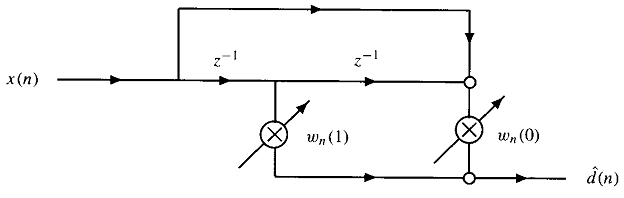
\includegraphics[width=7cm]{../TSM_StatDig/bilder/linear_phase_fir.png}
How a linear phase FIR filter 2 order is implemented in hardware.
\end{minipage}
\subsection{Wiener IIR Filter}
\begin{minipage}{8cm}
\subsubsection{Noncausal \hayes{353}}
\begin{tabbing}
Wiener-Hopf equations: \=
$H(e^{jw})=\frac{P_{dx}(e^{jw})}{P_{x}(e^{jw})}  \Rightarrow
\frac{P_{d}(e^{jw})}{P_{d}(e^{jw}) + P_{v}(e^{jw})}= \frac{SNR(e^{j\omega})}{SNR(e^{j\omega}) + 1}$ (often called \textbf{the} Wiener Filter) \\

Correlations: \>
	$r_x(k) =E \{ x(n)x^{*}(n-k) \} $\\
	\>$r_{dx}(k) =E\{d(n)x^{*}(n-k)\}$\\


Minimum Error:\>
	$\xi_{min} =r_d(0)-\sum \limits_{l=-\infty}^\infty h(l)r_{dx}^{*}(l)
	=\frac{1}{2\pi}\int \limits_{-\pi}^\pi[P_d(e^{jw})-H(e^{jw})P_{dx}^{*}(e^{jw})]dw$\\
	\>$=r_d(0)-\frac{1}{2\pi}\int \limits_{-\pi}^\pi[H(e^{jw})P_{dx}^{*}(e^{jw})]dw$
\end{tabbing}

\end{minipage}

\subsubsection{Causal \hayes{358}}
\begin{tabbing}
Spectral Factorization: \=
$ P_x(z) = \sigma_0^2 Q(z) Q^*(z^{-1}) $\\

System function:\hspace{1.2cm}\>
	$H(z)=\frac{1}{\sigma_0^2 Q(z) } [\frac{P_{dx}(z)}{Q^*(z^{-1})} ]_+ $ \\

Minimum Error:\>$\xi_{min} =r_d(0)-\sum \limits_{l=0}^\infty h(l)r_{dx}^{*}(l)
	=\frac{1}{2\pi}\int \limits_{-\pi}^\pi[P_d(e^{jw})-H(e^{jw})P_{dx}^{*}(e^{jw})]dw$\\

\end{tabbing}
Example \hayes{362}

\subsubsection{Linear Prediction IIR \hayes{365}}
\begin{tabbing}
System function:\hspace{0.2cm}\=
	$ r_{dx}(k)=r_x(k+\alpha)  \qquad \alpha \text{ = steps to predict.} $\\
\>	$ H(z)= \frac{1}{Q(z)}[z^\alpha Q(z)]_+ $ \hspace{6.8cm} \=$\rightarrow \text{monic, one step } H(z) = z [1- \frac{1}{Q(z)}] $\\
Minimum Error:\>
	$\xi_{min} =r_d(0)-\sum \limits_{l=0}^\infty h(l)r_{dx}^{*}(l)
		=\frac{1}{2\pi}\int \limits_{-\pi}^\pi[P_d(e^{jw})-H(e^{jw})P_{dx}^{*}(e^{jw})]dw $\>$ \rightarrow \text{monic, one step } \xi_{min} = \sigma^2_0$\\
\end{tabbing}


\subsubsection{Wiener Deconvolution \hayes{369}}
Deconvolutate a signal $x(n)=d(n)\ast g(n) + w(n)$ (not $x(n)=d(n) + g(n)$) it's not easy. At the best, the signal could be reconstruct as:
$\hat{D}(e^{\omega})=D(e^{j\omega}) + \frac{W(e^{j\omega})}{G(e^{j\omega})}=D(e^{j\omega})+V(e^{j\omega})$ \quad $V(e^{j\omega})$ isn't anymore white noise.
Espacialy if $G(e^{j\omega})$ becomes small the noise will be amplified.\\
System function:\hspace{1.2cm}
	$ H(z)= \frac{1}{G(z)}\left[\frac{P_d(z)}{P_d(z)+P_w(z)/|G(z)|^2}\right]$\\


\subsection{Discrete Kalman Filter}
The Kalman Filter is a Best Linear Unbiased Estimator (BLUE).

\textbf{Basic Idea}: The Kalman Filter estimates the Kalman Gain based on
the least squares error. Specifically, the Kalman Filter defines measurement values
using state variables and a noise signal. \\
\subsubsection{Prerequisites}
\begin{itemize}
	\item A physical model/system description.
	\item Measurement values, sensor fusion possible (multiple measurements for one
	system state).
	\item For standard Kalman: linear relationship between measurement values and
	state variables.
\end{itemize}


\subsubsection{Kalman Algorithm}

State and observation vectors:
\vspace{-0.2cm}
\begin{alignat*}{2}
	& \mathbf{x} \quad && p \times 1 \quad \text{state vector, can be chosen as seen fit} \\
	& \mathbf{\hat x}(a|b) \quad && \text{estimate of } \mathbf{x} \text{ at iteration } a \text{, given iterations up to } b
		\text{, needs to be initialized: } \mathbf{\hat x}(0|0)\\
	& \mathbf{y} \quad && q \times 1 \quad \text{observation vector (measured signals)}
\end{alignat*}
\vspace{-0.5cm}

Matrices given by the system (should be known):
\vspace{-0.2cm}
\begin{alignat*}{2}
	& \mathbf{A} \quad && p \times p \quad \text{state transition matrix} \\
	& \mathbf{C} \quad && q \times p \quad \text{observation matrix} \\
	& \mathbf{Q}_w \quad && p \times p \quad \text{noise covariance matrix for generating noise } \mathbf{w}(n) \\
	& \mathbf{Q}_v \quad && q \times q \quad \text{noise covariance matrix for measurement noise } \mathbf{v}(n)
\end{alignat*}
\vspace{-0.5cm}

Iteratively updated matrices:
\vspace{-0.2cm}
\begin{alignat*}{2}
	& \mathbf{P} \quad && p \times p \quad \text{error covariance matrix, needs to be initialized: } \mathbf{P}(0|0) \\
	& \mathbf{K} \quad && p \times q \quad \text{Kalman gain matrix}
\end{alignat*}
\vspace{-0.5cm}

\begin{alignat*}{2}
    &\text{State equation:}\qquad&&\mathbf{x}(n) =\mathbf{A}(n-1)\mathbf{x}(n-1) + \mathbf{w}(n) \nonumber\\
    &\text{Observation equation:}\qquad&&\mathbf{y}(n) =\mathbf{C}(n)\mathbf{x}(n) + \mathbf{v}(n) \nonumber\\
    \nonumber\\
    &\text{Initialization:}    \qquad    &&\mathbf{\hat x}(0|0)=E\{\mathbf{x}(0)\} \qquad \qquad \qquad \, \text{zero if no better guess}\nonumber\\
                                        &&&\mathbf{P}(0|0)=E\{\mathbf{e}(0|0)\mathbf{e}^{\mathrm H}(0|0)\} \qquad \text{usually a large diagonal matrix (= estimate is uncertain)}\nonumber\\
    \nonumber\\
    &\text{Prediction:}            \qquad    &&\mathbf{\hat{x}}(n|n-1)=\mathbf{A}(n-1)\mathbf{\hat{x}}(n-1|n-1)\\
                                        &&&\mathbf{P}(n|n-1)=\mathbf{A}(n-1)\mathbf{P}(n-1|n-1)\mathbf{A}^{\mathrm H}(n-1) + \mathbf{Q}_w(n)\\
    \nonumber\\
    &\text{Update:}                \qquad    &&\mathbf{K}(n)=\mathbf{P}(n|n-1)\mathbf{C}^{\mathrm H}(n)\left[\mathbf{C}(n) \mathbf{P}(n|n-1)\mathbf{C}^{\mathrm H}(n)+\mathbf{Q}_v(n)\right]^{-1}\\
                                        &&&\mathbf{\hat{x}}(n|n)=\mathbf{\hat{x}}(n|n-1)+\mathbf{K}(n)\left[\mathbf{y}(n)-\mathbf{C}(n)\mathbf{\hat{x}}(n|n-1)\right]\\
                                        &&&\mathbf{P}(n|n)=\left[\mathbf{I}-\mathbf{K}(n)\mathbf{C}(n)\right]\mathbf{P}(n|n-1)\\
                                        &&&\text{continue with prediction for next step}
\end{alignat*}

The steady-state is reached when $\mathbf{P}(n|n) = \mathbf{P}(n-1 | n-1)$ and $\mathbf{K}(n) = \mathbf{P}(n|n)$.

\subsubsection{Simplified Principle of the Kalman Filter}
\begin{minipage}{14.5cm}
Given two inaccurate sensors $T_1$ and $T_2$ (uncorrelated), measuring the same signal with known standard deviations $\sigma_1$ and $\sigma_2$. The best
estimator $\hat{T}$ is calculated as follows:\\
\end{minipage}
\hspace{0.25cm}
\begin{minipage}{5cm}
$\hat{T}=\frac{\sigma_1^2}{\sigma_1^2+\sigma_2^2}\cdot T_2+\frac{\sigma_2^2}{\sigma_1^2+\sigma_2^2}\cdot T_1$
\end{minipage}
\begin{minipage}{14.5cm}
Given two correlated signals $T_1$ and $T_2$ with known $\sigma_1$, $\sigma_2$, and the correlation coefficient $\rho$. The best
estimator $\hat{T}$ is calculated as follows:\\
\end{minipage}
\hspace{0.25cm}
\begin{minipage}{5cm}
$\hat{T}=k_1\cdot T_1 + k_2\cdot T_2$\\
$k_1=\frac{\sigma_2^2-\rho \sigma_1 \sigma_2}{\sigma_1^2 - 2 \rho \sigma_1 \sigma_2 + \sigma_2^2}$\\
$k_2=1-k_1=\frac{\sigma_1^2-\rho \sigma_1 \sigma_2}{\sigma_1^2 - 2 \rho \sigma_1 \sigma_2 + \sigma_2^2}$\\
\end{minipage}


\subsubsection{Kalman Modelling of Known System Behaviour}
When a system has known behaviour, the state space representation can be used to find the Kalman matrices. The system is interpreted as a measurement with input $w(n)$ (measurement noise), output $y(n)$ and an added process noise $v(n)$ that is directly added to $y(n)$.

\begin{longtable}[H]{|>{\bfseries}p{0.3\textwidth}|p{0.65\textwidth}|}
	\hline
	1.: General transfer function:
		& $H(z) = \dfrac{Y(z)}{W(z)} = \dfrac{b_0 + b_1z^{-1} + b_2 z^{-2} + \dots + b_q z^{-q}}{1 + a_1z^{-1} + a_2 z^{-2} + \dots + a_p z^{-p}}$\\
		& \color{red}{Warning: The z-Transform of a known model does not always yield the correct difference equation! For example if a pole is on the unit circle\newline e.g $y(n) = (-1)^n \FT \frac{1}{1+z^{-1}} \IFT y(n) \neq 1 - y(n-1)$.\newline \textrightarrow What you need to do is to find the difference equation! The z-Transform might be one way to do that, but it doesn't always work.}\\
	\hline
	2.: Difference equation:
		& $y(n) = v(n) + b_0 w(n) + \ldots + b_q w(n-q) - a_1y(n-1) + \ldots - a_q y(n-q)$\\
	\hline
	3.: States:
		& {\begin{align*}
				x(n) 	&= w(n) - a_1 x(n-1) - a_2 x(n-2) - \ldots - a_p x(n-p)\\
				x(n-1)	&= x(n-1)\\
				\vdots 	&=	\vdots\\
				x(n-max(p,q) &= x(n-max(p,q))\\
		\end{align*}}\\
		& For more information see \href{https://github.com/HSR-Stud/DigSig2}{DigSig2 cheat sheet section 1.2 Canonical Form}. (Flow diagram and states)\\
	\hline
	4.: State space representation:
		& $A = \begin{bmatrix}
			-a_1 	& -a_2 		& \dots 	& -a_{p-1}	& -a_p\\
			1		& 0			& \dots		& 0			& 0\\
			0		& 1			& \dots		& 			& 0\\
			\vdots	& \vdots	& \ddots	& \vdots	& 0\\
			0		& 0			& \dots		& 1			& 0\\
		\end{bmatrix},
		B = \begin{bmatrix}
			w(n)\\
			0\\
			0\\
			\vdots\\
			0\\
		\end{bmatrix}$\\
		& $C = \begin{bmatrix}
			b_0 & b_1 & \dots & b_q\
		\end{bmatrix}, D = v(n)$\\
	\hline
\end{longtable}
